\chapter{\ifenglish Testing and Quality Assurance\else การทดสอบและการรับรองคุณภาพ\fi}

\section{การทดสอบและการรับรองคุณภาพทางวิศวกรรม}

\subsection{กลยุทธ์และเครื่องมือทดสอบ}

\begin{itemize}[leftmargin=1.8em, itemsep=3pt]
  \item \textbf{Unit Test} --- ทดสอบฟังก์ชัน เมธอด และคลาสแยกตามหน่วยการทำงาน
  \item \textbf{Integration Test} --- ทดสอบการทำงานร่วมกันของหลายคอมโพเนนต์
  \item \textbf{Load Test} --- ทดสอบประสิทธิภาพของระบบภายใต้ภาระงาน เช่น จำนวนผู้ใช้พร้อมกัน, response time, throughput และความเสถียรของระบบ
\end{itemize}

\renewcommand{\arraystretch}{1.3}
\begin{tabularx}{\linewidth}{lX}
  \toprule
  \textbf{เครื่องมือ} & \textbf{วัตถุประสงค์}\\
  \midrule
  Vitest                & Test Runner สำหรับ Unit และ Integration Test ที่รวดเร็ว\\
  React Testing Library & ทดสอบ UI ระดับ Component\\
  jsdom                 & จำลองสภาพแวดล้อม Browser\\
  Grafana               & จำลองภาระงานผู้ใช้เพื่อทดสอบ Load/Performance ของระบบ\\
  Prometheus            & เก็บรวบรวม Metrics เช่น CPU, Memory, Latency\\
  \bottomrule
\end{tabularx}

\subsection{ผลการทดสอบ}

\begin{figure}[H]
  \centering
  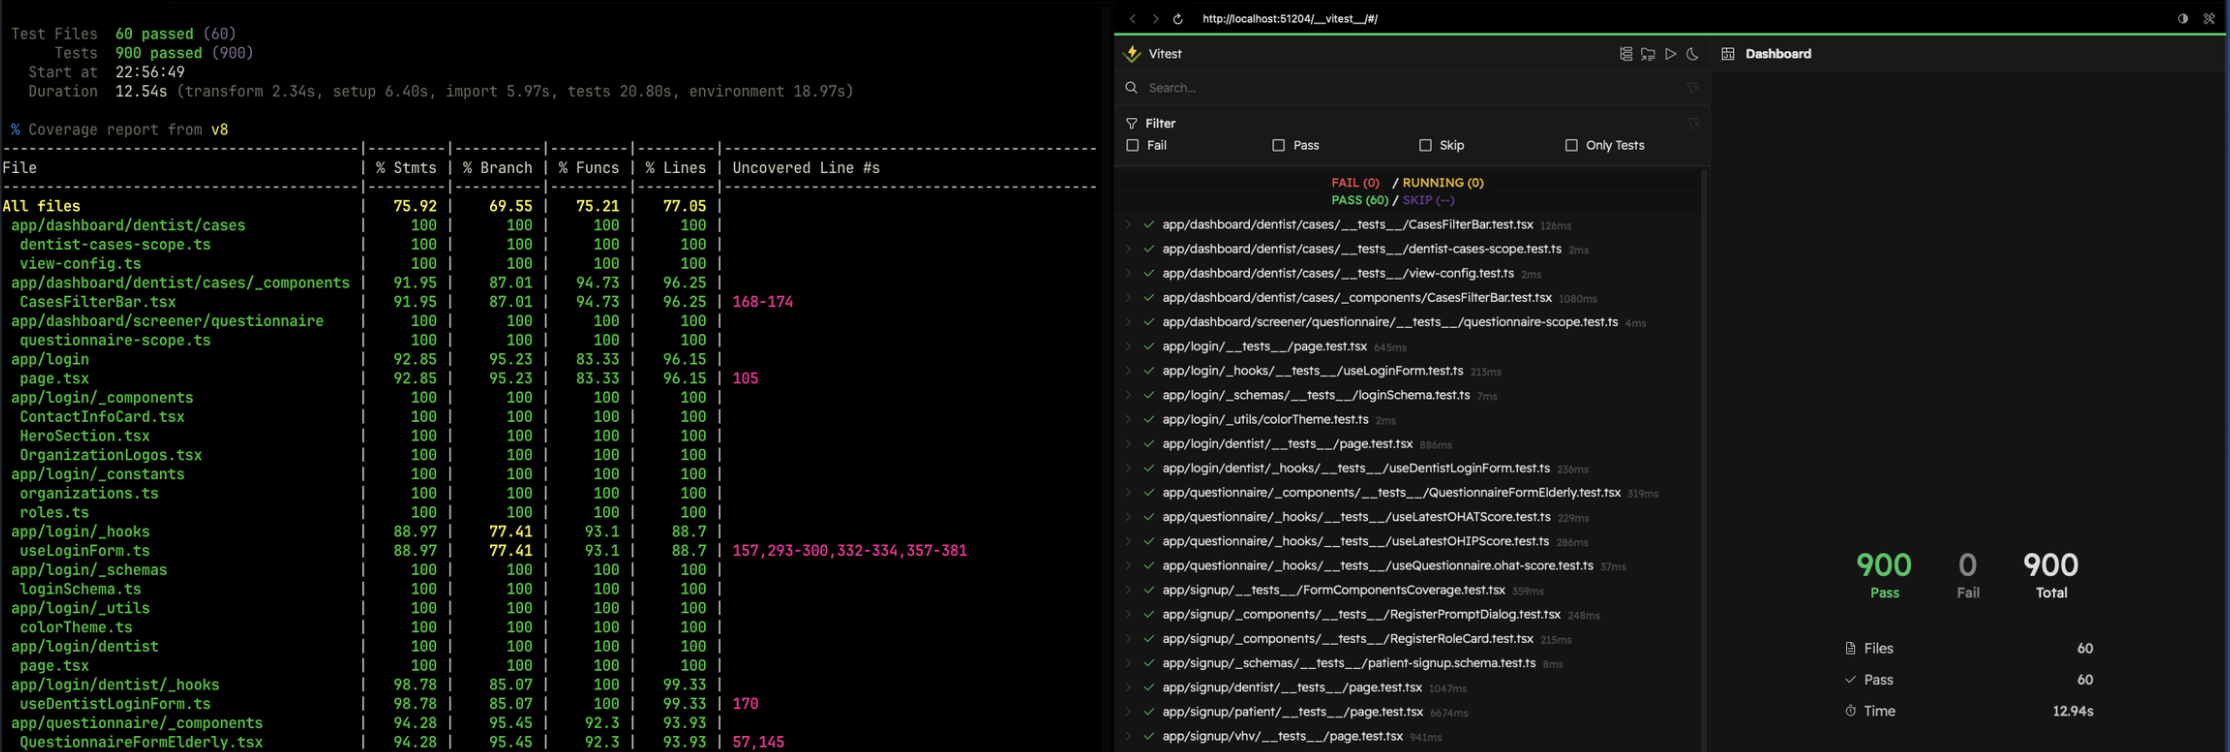
\includegraphics[width=\linewidth]{images/4.1.2.png}
  \caption{ผลการทดสอบ Unit/Integration: Coverage Report และ Vitest UI
    (900 passed, 0 failed) โดยรันเสร็จภายใน $<13\,\text{s}$}
\end{figure}

\begin{tcolorbox}[greenbox]
  \renewcommand{\arraystretch}{1.4}
  \begin{tabularx}{\linewidth}{Xl}
    \textbf{จำนวน Test ทั้งหมด} & 900 (Unit + Integration)\\
    \textbf{สถานะ} & \textcolor{successgreen}{\textbf{ผ่าน 100\%}}\\
    \textbf{Code Coverage} & $\approx$75\%\\
    \textbf{Critical Logic} & \textbf{100\%}\\
    \textbf{เวลาในการทดสอบ} & $<13\,\text{s}$\\
  \end{tabularx}
\end{tcolorbox}

% =========================
\subsection{โปรไฟล์ภาระงานสังเคราะห์ (Synthetic Load)}

\begin{tcolorbox}[bluebox,title={สรุปผล Synthetic Load}]
  \renewcommand{\arraystretch}{1.35}
  \begin{tabularx}{\linewidth}{Xl}
    \textbf{ระยะเวลา} & 1 ชั่วโมง\\
    \textbf{จำนวน Request} & 7,632\\
    \textbf{ค่าเฉลี่ย RPS} & 2.12\\
    \textbf{Success Rate} & 99.46\%\\
  \end{tabularx}
\end{tcolorbox}

\begin{figure}[H]
  \centering
  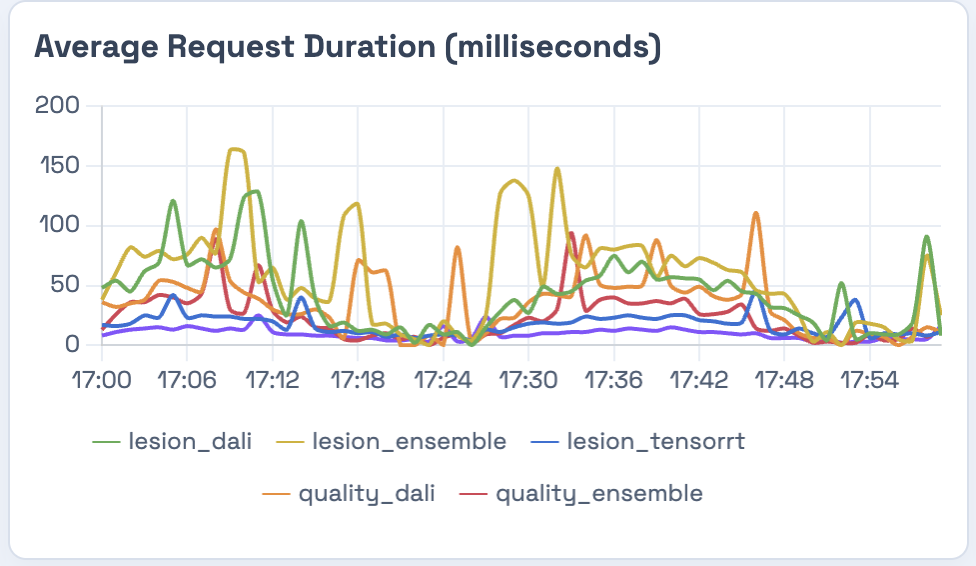
\includegraphics[width=\linewidth]{images/4.1.png}
  \caption{Request Duration}
\end{figure}

\begin{figure}[H]
  \centering
  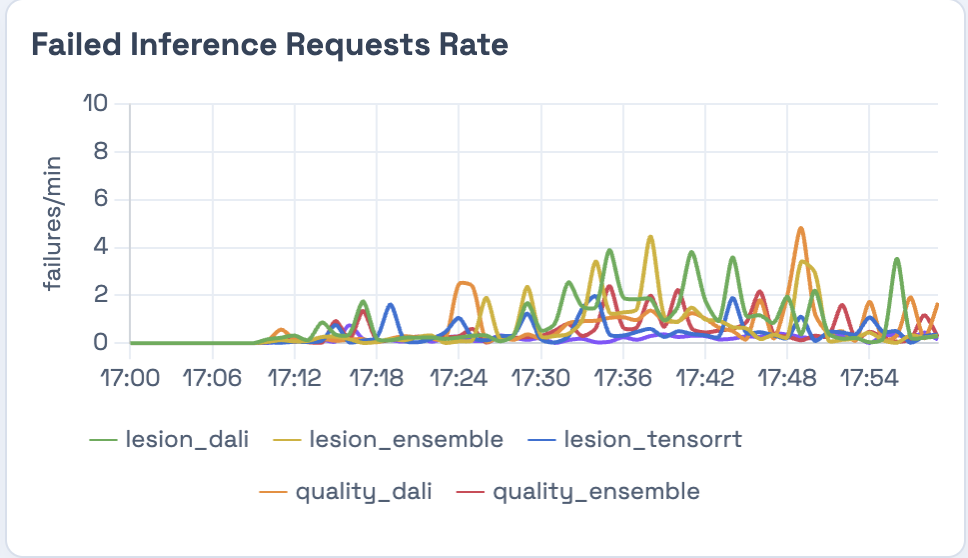
\includegraphics[width=\linewidth]{images/4.2.png}
  \caption{Failed Requests}
\end{figure}

\begin{figure}[H]
  \centering
  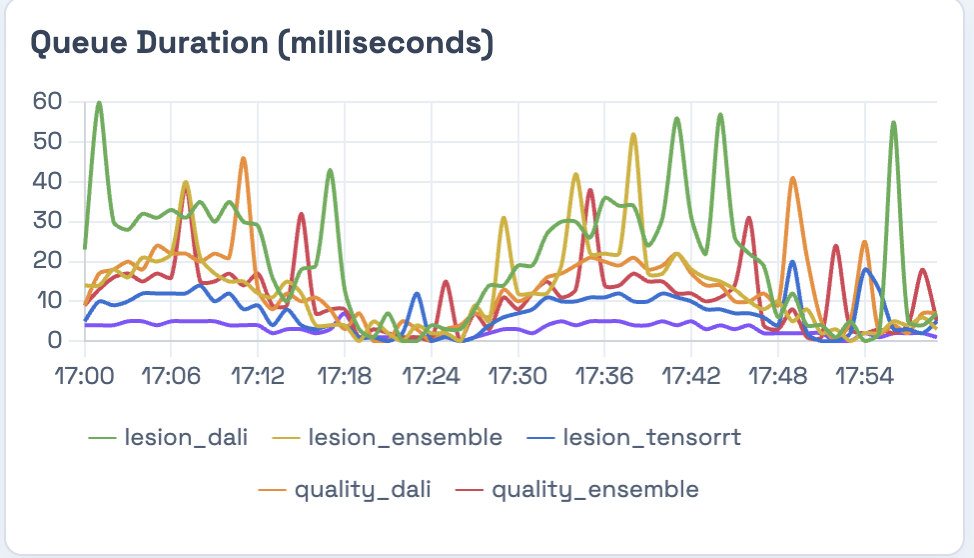
\includegraphics[width=\linewidth]{images/4.3.png}
  \caption{Queue Time}
\end{figure}

\begin{figure}[H]
  \centering
  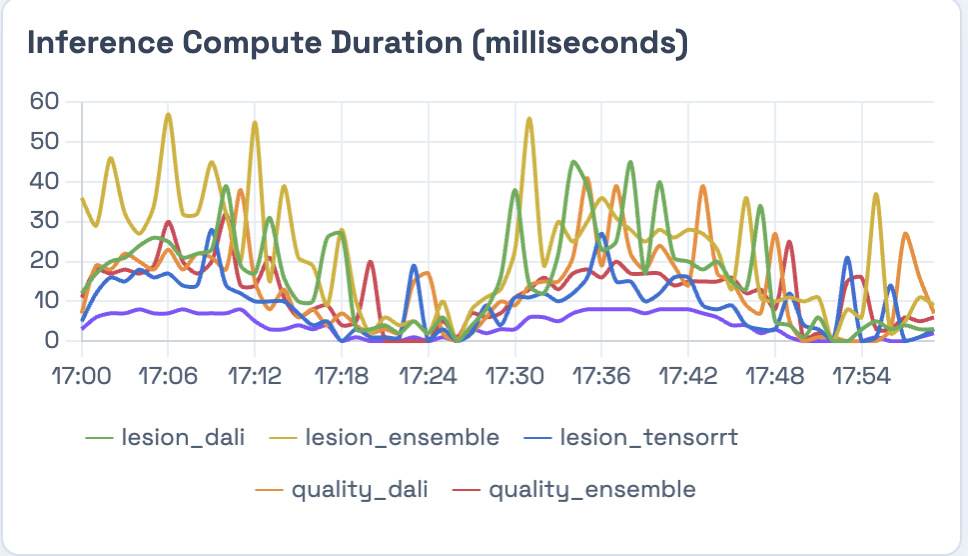
\includegraphics[width=\linewidth]{images/4.4.png}
  \caption{Compute Time}
\end{figure}

\begin{figure}[H]
  \centering
  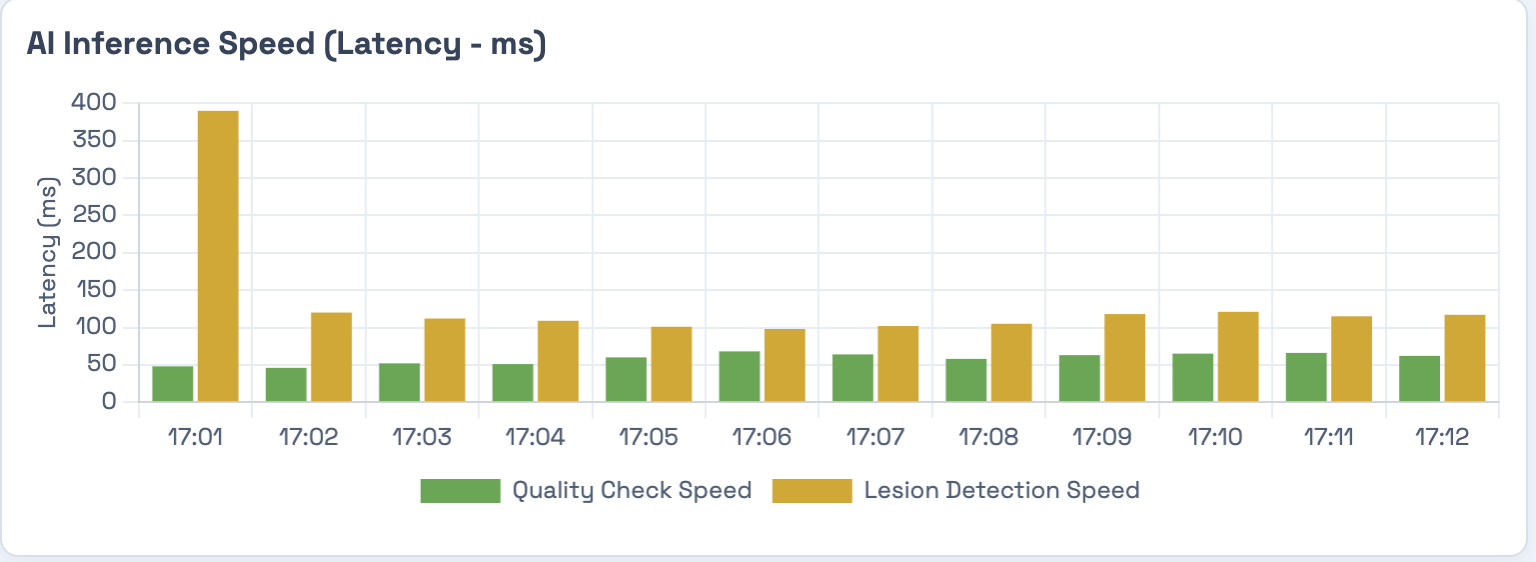
\includegraphics[width=\linewidth]{images/4.5.png}
  \caption{AI Inference Latency}
\end{figure}

% =========================
\subsection{การวิเคราะห์ผลการทดสอบ}

จากผลการทดสอบพบว่า ระบบมีอัตราความสำเร็จสูงถึง 99.46\% ซึ่งสะท้อนถึงความเสถียรภายใต้ภาระงานต่อเนื่อง

แม้ค่า RPS จะไม่สูงมาก แต่สอดคล้องกับลักษณะการใช้งานจริงในระดับชุมชน ซึ่งไม่ได้มีรูปแบบการใช้งานหนาแน่นเช่นระบบขนาดใหญ่

นอกจากนี้ ค่า latency และ queue time ที่ต่ำ แสดงให้เห็นว่าระบบสามารถจัดการคำขอได้อย่างมีประสิทธิภาพ และไม่เกิด bottleneck ใน pipeline

% =========================
\section{การอภิปรายผล}

จากผลการทดสอบพบว่า ความสำเร็จของระบบไม่ได้ขึ้นอยู่กับ AI เพียงอย่างเดียว แต่เกิดจากการออกแบบระบบโดยรวม ทั้งด้านสถาปัตยกรรม workflow และ usability

การใช้ Modular Monolith Architecture และ Dual-Path AI ช่วยเพิ่มความเสถียรและลดความเสี่ยงจากการล่มของระบบ ซึ่งเป็นปัจจัยสำคัญในระบบทางการแพทย์

นอกจากนี้ การออกแบบ workflow ให้สอดคล้องกับการทำงานจริงของบุคลากร เช่น อสม. และทันตแพทย์ มีบทบาทสำคัญในการทำให้ระบบสามารถใช้งานจริงได้

อย่างไรก็ตาม ยังมีข้อจำกัด เช่น การพึ่งพา AI จากภายนอก และการทดสอบที่ยังอยู่ในระดับนำร่อง

% =========================
\section{สรุปผลการดำเนินงาน}

ระบบ eDENT-ELDER Phase 2 สามารถทำงานได้ครบถ้วนตามวัตถุประสงค์ และมีศักยภาพในการนำไปใช้งานจริง

ระบบสามารถเพิ่มการเข้าถึงบริการ ลดภาระของบุคลากร และเพิ่มประสิทธิภาพในการตรวจพบโรคในระยะเริ่มต้น

ผลการทดสอบทั้งด้าน functional และ performance ยืนยันถึงความพร้อมของระบบสำหรับการใช้งานจริงในระดับบริการ